\documentclass[11pt, a4paper]{article}

\usepackage[a4paper, top=2.5cm, bottom=2.5cm, left=2cm, right=2cm]{geometry}
\usepackage[T1]{fontenc}
\usepackage[english]{babel}

\usepackage{amsmath}
\usepackage{amssymb}
\usepackage{booktabs}
\usepackage{array}
\usepackage{graphicx}
\usepackage{tikz}
\usepackage{tikz-3dplot}
\usetikzlibrary{calc, arrows.meta, angles, quotes}
\usepackage{hyperref}

\title{\textbf{Coil Sensitivity Analysis}}
\author{Kevin Ying}
\date{\today}

\begin{document}

\maketitle
\section{Background: Magnetic Field Modeling}

Consider an array of $4 \times 4$ electromagnetic sub-coils. Each sub-coil $(i,j)$ is located at position $\mathbf{p}_{i,j} \in \mathbb{R}^3$ with orientation unit vector $\mathbf{n}_{i,j} \in \mathbb{S}^2$, as depicted in Figure~\ref{fig:solenoid_dipole}. Each coil is driven by an AC current $I_{i,j}(t)$, defined by:
\begin{equation}
    I_{i,j}(t) = I_0 \cos(\omega t + \psi_{i,j}),
\end{equation}
where $I_0$ is the peak AC current amplitude, $\omega$ is the drive angular frequency, and $\psi_{i,j}$ is the relative actuation phase shift of coil $(i,j)$.

\begin{figure}[htbp]
\centering
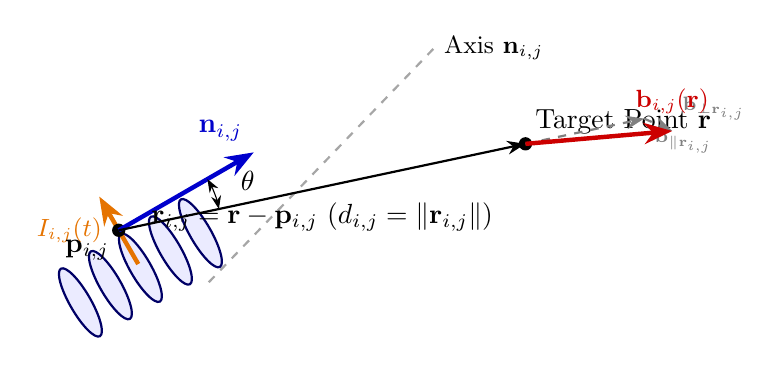
\begin{tikzpicture}[scale=1.1, >=Stealth]
    % Coordinates
    \coordinate (P) at (0,0);
    \coordinate (N_axis) at (30:2.5);
    \coordinate (R) at (12:4.8);
    
    % Axis line through solenoid
    \draw[dashed, gray!70, thick] (-30:1.2) -- (30:4.2) node[right, black, font=\small] {Axis $\mathbf{n}_{i,j}$};
    
    % Draw Solenoid / Sub-coil loops
    \begin{scope}[rotate=30]
        \foreach \x in {-0.8, -0.4, 0.0, 0.4, 0.8} {
            \draw[thick, fill=blue!8, draw=blue!40!black] (\x, -0.5) ellipse (0.12 and 0.45);
        }
        % Current direction arrow
        \draw[->, ultra thick, orange!90!black] (0.0, -0.45) -- (0.0, 0.45) node[midway, left=2pt, font=\small] {$I_{i,j}(t)$};
    \end{scope}

    % Center point p_{i,j}
    \filldraw[black] (P) circle (2pt) node[below left] {$\mathbf{p}_{i,j}$};
    
    % Orientation Unit Vector n_{i,j}
    \draw[->, ultra thick, blue!80!black] (P) -- (30:1.8) node[above left] {$\mathbf{n}_{i,j}$};

    % Target Point r
    \filldraw[black] (R) circle (2pt) node[above right] {Target Point $\mathbf{r}$};

    % Displacement vector r_{i,j}
    \draw[->, thick, black] (P) -- (R) node[midway, below=2pt] {$\mathbf{r}_{i,j} = \mathbf{r} - \mathbf{p}_{i,j}$ ($d_{i,j} = \|\mathbf{r}_{i,j}\|$)};

    % Angle theta between n_{i,j} and r_{i,j}
    \coordinate (N_pt) at (30:1.8);
    \draw pic[draw, <->, "$\theta$", angle radius=1.3cm, angle eccentricity=1.35] {angle = R--P--N_pt};

    % Decomposed Magnetic Field at Point R
    \coordinate (B_end) at ($(R) + (5:1.7)$);
    \coordinate (B_par) at ($(R) + (12:1.4)$);

    \draw[->, thick, dashed, gray] (R) -- (B_par) node[below right, font=\scriptsize] {$\mathbf{b}_{\parallel \mathbf{r}_{i,j}}$};
    \draw[->, thick, dashed, gray] (B_par) -- (B_end) node[above right, font=\scriptsize] {$\mathbf{b}_{\perp \mathbf{r}_{i,j}}$};
    \draw[->, ultra thick, red!80!black] (R) -- (B_end) node[above=2pt, font=\small] {$\mathbf{b}_{i,j}(\mathbf{r})$};
\end{tikzpicture}
\caption{Geometry of a single sub-coil $(i,j)$ located at position $\mathbf{p}_{i,j}$ with orientation unit vector $\mathbf{n}_{i,j}$ driven by time-varying current $I_{i,j}(t)$, generating magnetic field response $\mathbf{b}_{i,j}(\mathbf{r})$ at target point $\mathbf{r}$.}
\label{fig:solenoid_dipole}
\end{figure}

Under the point-dipole approximation, the magnetic flux density response per unit current generated by sub-coil $(i,j)$ at target point $\mathbf{r} \in \mathbb{R}^3$ is given by:
\[
    \mathbf{b}_{i,j}(\mathbf{r}) = K_{\text{dipole}} \left( \frac{3 (\mathbf{r}_{i,j} \cdot \mathbf{n}_{i,j}) \mathbf{r}_{i,j}}{d_{i,j}^5} - \frac{\mathbf{n}_{i,j}}{d_{i,j}^3} \right),
\]
where $\mathbf{r}_{i,j} = \mathbf{r} - \mathbf{p}_{i,j}$ is the relative position vector, $d_{i,j} = \|\mathbf{r}_{i,j}\|$ is the Euclidean distance, and $K_{\text{dipole}} = \frac{\mu_0 m_0}{4\pi}$ represents the unit-current magnetic dipole strength prefactor ($m_0 = N A$ for a coil with $N$ turns and effective cross-sectional area $A$).

Applying linear superposition across all 16 driven coils and expanding $I_{i,j}(t)$ using the cosine angle addition identity gives the total time-varying field $\mathbf{B}(\mathbf{r}, t)$:
\[
    \mathbf{B}(\mathbf{r}, t) = \sum_{i=1}^4 \sum_{j=1}^4 \mathbf{b}_{i,j}(\mathbf{r}) I_{i,j}(t) = \mathbf{u}(\mathbf{r}) \cos(\omega t) + \mathbf{v}(\mathbf{r}) \sin(\omega t),
\]
where the spatial field is resolved into orthogonal in-phase $\mathbf{u}(\mathbf{r})$ and $90^\circ$-lagged (quadrature) $\mathbf{v}(\mathbf{r})$ vector components:
\[
    \mathbf{u}(\mathbf{r}) = I_0 \sum_{i=1}^4 \sum_{j=1}^4 \mathbf{b}_{i,j}(\mathbf{r}) \cos\psi_{i,j}, \qquad 
    \mathbf{v}(\mathbf{r}) = -I_0 \sum_{i=1}^4 \sum_{j=1}^4 \mathbf{b}_{i,j}(\mathbf{r}) \sin\psi_{i,j}.
\]

From $\mathbf{u}(\mathbf{r})$ and $\mathbf{v}(\mathbf{r})$, the field rotation vector $\mathbf{w}(\mathbf{r})$, local rotation axis $\mathbf{n}_{\text{rot}}(\mathbf{r})$, root-mean-square (RMS) field magnitude $B_{\text{rms}}(\mathbf{r})$, and lateral magnetic force driver gradient $\mathbf{g}_{\text{lat}}(\mathbf{r})$ are computed as:
\[
    \mathbf{w}(\mathbf{r}) = \mathbf{u}(\mathbf{r}) \times \mathbf{v}(\mathbf{r}), \qquad \mathbf{n}_{\text{rot}}(\mathbf{r}) = \frac{\mathbf{w}(\mathbf{r})}{\|\mathbf{w}(\mathbf{r})\|},
\]
\[
    B_{\text{rms}}(\mathbf{r}) = \sqrt{\frac{1}{2} \left( \|\mathbf{u}(\mathbf{r})\|^2 + \|\mathbf{v}(\mathbf{r})\|^2 \right)}, \qquad \mathbf{g}_{\text{lat}}(\mathbf{r}) = \nabla_{xy} \left( B_{\text{rms}}^2(\mathbf{r}) \right).
\]

\section{Frames and Kinematics in $\mathfrak{se}(3)$}
We define frames and sub-coil poses using homogeneous transformation matrices $T_{i,j} \in SE(3)$, parameterized by rotation matrix $R_{i,j} \in SO(3)$ (where $\mathbf{n}_{i,j} = R_{i,j} \mathbf{e}_z$) and translation vector $\mathbf{p}_{i,j} \in \mathbb{R}^3$:
\[
    T_{i,j} = \begin{bmatrix} R_{i,j} & \mathbf{p}_{i,j} \\ \mathbf{0}^T & 1 \end{bmatrix}.
\]
When performing operations across frame transformations, matrix compositions combine both components directly:
\[
    T_{W \gets C_i} = \mathrm{Rot}_Z(\Phi_i) \, T_{W \gets C_1}, \qquad \mathbf{p}_{i,j} = R_i \mathbf{p}^{(t)}_j, \qquad \mathbf{n}_{i,j} = R_i \mathbf{n}^{(t)}_j.
\]

\section{Additive Gaussian Pose Noise}
For each coil pose $T_{i,j}$, we apply additive zero-mean Gaussian noise $\boldsymbol{\xi}_{i,j} = [\boldsymbol{\omega}_{i,j}^T, \boldsymbol{\nu}_{i,j}^T]^T \in \mathfrak{se}(3)$:
\[
    \boldsymbol{\xi}_{i,j} \sim \mathcal{N}(\mathbf{0}, \boldsymbol{\Sigma}_{\xi}), \qquad \boldsymbol{\Sigma}_{\xi} = \text{diag}(\sigma_{\text{rot}}^2 \mathbf{I}_3, \sigma_{\text{trans}}^2 \mathbf{I}_3).
\]
To first order, position perturbations $\delta \mathbf{p}_{i,j}$ and orientation perturbations $\delta \mathbf{n}_{i,j}$ follow:
\[
    \delta \mathbf{p}_{i,j} = \boldsymbol{\nu}_{i,j}, \qquad \delta \mathbf{n}_{i,j} = \boldsymbol{\omega}_{i,j} \times \mathbf{n}_{i,j} = -\hat{\mathbf{n}}_{i,j} \boldsymbol{\omega}_{i,j},
\]
where $\hat{\mathbf{a}}$ denotes the $3 \times 3$ skew-symmetric cross-product matrix of vector $\mathbf{a}$:
\[
    \hat{\mathbf{a}} = \begin{bmatrix} 0 & -a_z & a_y \\ a_z & 0 & -a_x \\ -a_y & a_x & 0 \end{bmatrix}.
\]

\section{Objective Function Formulation}
We formulate general cost terms integrated over a 2D/3D region of interest $\Omega$:
\[
    \mathcal{J}_{\text{sens}} = \int_{\Omega} \sum_{i=1}^4 \sum_{j=1}^4 \text{Tr}\left( \mathbf{J}_{i,j}^{\mathbf{n}_{\text{rot}}}(\mathbf{r}) \boldsymbol{\Sigma}_{\xi} \left(\mathbf{J}_{i,j}^{\mathbf{n}_{\text{rot}}}(\mathbf{r})\right)^T \right) d\mathbf{r},
\]
\[
    \mathcal{J}_{\text{mag}} = -\int_{\Omega} B_{\text{rms}}(\mathbf{r}) \, d\mathbf{r}, \qquad \mathcal{J}_{\text{grad}} = \int_{\Omega} \|\mathbf{g}_{\text{lat}}(\mathbf{r})\|^2 \, d\mathbf{r}.
\]
We investigate coupled coil plates versus individually movable coil designs, and model perturbations individually as follows:
\begin{itemize}
    \item \textbf{Coupled Coil Plates:} Mechanical noise cascades through the assembly. Variance is added at the cluster baseplate level ($\boldsymbol{\Sigma}_{\text{plate}}$) as well as the individual sub-coil mounts ($\boldsymbol{\Sigma}_{\text{coil}}$), doubling total variance ($\boldsymbol{\Sigma}_{\xi} = \boldsymbol{\Sigma}_{\text{plate}} + \boldsymbol{\Sigma}_{\text{coil}} \approx 2\boldsymbol{\Sigma}_{\text{coil}}$).
    \item \textbf{Individually Mounted Coils:} Each sub-coil is positioned independently, resulting in single-level noise ($\boldsymbol{\Sigma}_{\xi} = \boldsymbol{\Sigma}_{\text{coil}}$).
\end{itemize}

\section{Perturbation Propagation}

To implement this sensitivity framework in symbolic optimization tools like CasADi, we physically derive the exact closed-form Jacobians mapping $\mathfrak{se}(3)$ perturbations $\boldsymbol{\xi}_{i,j}$ to the rotation axis variation $\delta \mathbf{n}_{\text{rot}}(\mathbf{r})$.

\subsection{Physical Derivation of Single-Coil Flux Density Sensitivity}
Consider the dipole response $\mathbf{b}_{i,j}(\mathbf{r})$. Taking the total differential with respect to position vector $\mathbf{p}_{i,j}$ and unit normal vector $\mathbf{n}_{i,j}$ gives:
\[
    \delta \mathbf{b}_{i,j} = \frac{\partial \mathbf{b}_{i,j}}{\partial \mathbf{p}_{i,j}} \delta \mathbf{p}_{i,j} + \frac{\partial \mathbf{b}_{i,j}}{\partial \mathbf{n}_{i,j}} \delta \mathbf{n}_{i,j}.
\]

\paragraph{1. Position Derivative Matrix ($\mathbf{J}_{\mathbf{p}_{i,j}}^{\mathbf{b}} \in \mathbb{R}^{3 \times 3}$):}
Since $\mathbf{r}_{i,j} = \mathbf{r} - \mathbf{p}_{i,j}$, taking spatial gradients with respect to $\mathbf{p}_{i,j}$ yields $\frac{\partial \mathbf{r}_{i,j}}{\partial \mathbf{p}_{i,j}} = -\mathbf{I}_3$ and $\frac{\partial d_{i,j}}{\partial \mathbf{p}_{i,j}} = -\frac{\mathbf{r}_{i,j}^T}{d_{i,j}}$. Differentiating $\mathbf{b}_{i,j}$ using product and chain rules yields:
\[
    \mathbf{J}_{\mathbf{p}_{i,j}}^{\mathbf{b}} = \frac{\partial \mathbf{b}_{i,j}}{\partial \mathbf{p}_{i,j}} = -K_{\text{dipole}} \left[ \frac{3 (\mathbf{r}_{i,j}^T \mathbf{n}_{i,j}) \mathbf{I}_3 + 3 \mathbf{r}_{i,j} \mathbf{n}_{i,j}^T + 3 \mathbf{n}_{i,j} \mathbf{r}_{i,j}^T}{d_{i,j}^5} - \frac{15 (\mathbf{r}_{i,j}^T \mathbf{n}_{i,j}) \mathbf{r}_{i,j} \mathbf{r}_{i,j}^T}{d_{i,j}^7} \right].
\]
\begin{itemize}
    \item $d_{i,j}^{-5}$: Accounts for second-order spatial decay of the magnetic gradient tensor.
    \item $d_{i,j}^{-7}$: Captures higher-order geometric dilation from distance perturbations along vector $\mathbf{r}_{i,j}$.
\end{itemize}

\paragraph{2. Orientation Derivative Matrix ($\mathbf{J}_{\boldsymbol{\omega}_{i,j}}^{\mathbf{b}} \in \mathbb{R}^{3 \times 3}$):}
Differentiating $\mathbf{b}_{i,j}$ with respect to coil normal vector $\mathbf{n}_{i,j}$ gives:
\[
    \frac{\partial \mathbf{b}_{i,j}}{\partial \mathbf{n}_{i,j}} = K_{\text{dipole}} \left[ \frac{3 \mathbf{r}_{i,j} \mathbf{r}_{i,j}^T}{d_{i,j}^5} - \frac{\mathbf{I}_3}{d_{i,j}^3} \right].
\]
Substituting the differential rotation kinematic relationship $\delta \mathbf{n}_{i,j} = -\hat{\mathbf{n}}_{i,j} \boldsymbol{\omega}_{i,j}$ into the total differential yields:
\[
    \mathbf{J}_{\boldsymbol{\omega}_{i,j}}^{\mathbf{b}} = \frac{\partial \mathbf{b}_{i,j}}{\partial \mathbf{n}_{i,j}} \frac{\partial \mathbf{n}_{i,j}}{\partial \boldsymbol{\omega}_{i,j}} = -K_{\text{dipole}} \left[ \frac{3 \mathbf{r}_{i,j} \mathbf{r}_{i,j}^T}{d_{i,j}^5} - \frac{\mathbf{I}_3}{d_{i,j}^3} \right] \hat{\mathbf{n}}_{i,j}.
\]

Concatenating both blocks forms the block flux density Jacobian $\mathbf{J}_{i,j}^{\mathbf{b}} = [\mathbf{J}_{\boldsymbol{\omega}_{i,j}}^{\mathbf{b}} \;\; \mathbf{J}_{\mathbf{p}_{i,j}}^{\mathbf{b}}] \in \mathbb{R}^{3 \times 6}$ such that $\delta \mathbf{b}_{i,j} = \mathbf{J}_{i,j}^{\mathbf{b}} \boldsymbol{\xi}_{i,j}$.

\subsection{Propagation to Time-Separated Field Vectors}
Because the total field is a linear combination of individual sub-coil fields weighted by current phase $\psi_{i,j}$, the variations in in-phase vector $\mathbf{u}(\mathbf{r})$ and lagging vector $\mathbf{v}(\mathbf{r})$ with respect to pose noise $\boldsymbol{\xi}_{i,j}$ are:
\[
    \frac{\partial \mathbf{u}}{\partial \boldsymbol{\xi}_{i,j}} = I_0 \cos\psi_{i,j} \mathbf{J}_{i,j}^{\mathbf{b}}, \qquad \frac{\partial \mathbf{v}}{\partial \boldsymbol{\xi}_{i,j}} = -I_0 \sin\psi_{i,j} \mathbf{J}_{i,j}^{\mathbf{b}}.
\]

\subsection{Cross-Product Propagation to Rotation Vector $\mathbf{w}(\mathbf{r})$}
The unnormalized rotation vector is defined as $\mathbf{w}(\mathbf{r}) = \mathbf{u}(\mathbf{r}) \times \mathbf{v}(\mathbf{r})$. Differentiating via the vector product rule gives:
\[
    \delta \mathbf{w} = \delta \mathbf{u} \times \mathbf{v} + \mathbf{u} \times \delta \mathbf{v} = -\mathbf{v} \times \delta \mathbf{u} + \mathbf{u} \times \delta \mathbf{v}.
\]
Converting cross products to skew-symmetric matrix multiplication ($-\mathbf{v} \times \delta \mathbf{u} = -\hat{\mathbf{V}} \delta \mathbf{u}$ and $\mathbf{u} \times \delta \mathbf{v} = \hat{\mathbf{U}} \delta \mathbf{v}$) yields the Jacobian $\mathbf{J}_{i,j}^{\mathbf{w}} = \frac{\partial \mathbf{w}}{\partial \boldsymbol{\xi}_{i,j}} \in \mathbb{R}^{3 \times 6}$:
\[
    \mathbf{J}_{i,j}^{\mathbf{w}} = -\hat{\mathbf{V}} \left( I_0 \cos\psi_{i,j} \mathbf{J}_{i,j}^{\mathbf{b}} \right) - \hat{\mathbf{U}} \left( I_0 \sin\psi_{i,j} \mathbf{J}_{i,j}^{\mathbf{b}} \right).
\]
\begin{itemize}
    \item $\hat{\mathbf{U}}, \hat{\mathbf{V}} \in \mathbb{R}^{3 \times 3}$: Skew-symmetric matrices constructed from field vectors $\mathbf{u}(\mathbf{r})$ and $\mathbf{v}(\mathbf{r})$.
\end{itemize}

\subsection{Projection to Unit Rotation Axis $\mathbf{n}_{\text{rot}}(\mathbf{r})$}
Differentiating the normalization operator $\mathbf{n}_{\text{rot}} = \frac{\mathbf{w}}{\|\mathbf{w}\|}$ with respect to vector $\mathbf{w}$ yields the orthogonal projection matrix $\mathbf{P}_{\mathbf{w}}^\perp$:
\[
    \frac{\partial \mathbf{n}_{\text{rot}}}{\partial \mathbf{w}} = \frac{1}{\|\mathbf{w}\|} \left( \mathbf{I}_3 - \frac{\mathbf{w} \mathbf{w}^T}{\|\mathbf{w}\|^2} \right) = \frac{1}{\|\mathbf{w}\|} \left( \mathbf{I}_3 - \mathbf{n}_{\text{rot}} \mathbf{n}_{\text{rot}}^T \right).
\]
Applying the chain rule gives the final composite Jacobian $\mathbf{J}_{i,j}^{\mathbf{n}_{\text{rot}}} = \frac{\partial \mathbf{n}_{\text{rot}}}{\partial \boldsymbol{\xi}_{i,j}} \in \mathbb{R}^{3 \times 6}$:
\[
    \mathbf{J}_{i,j}^{\mathbf{n}_{\text{rot}}} = \frac{1}{\|\mathbf{w}\|} \left( \mathbf{I}_3 - \mathbf{n}_{\text{rot}} \mathbf{n}_{\text{rot}}^T \right) \mathbf{J}_{i,j}^{\mathbf{w}}.
\]
This closed-form formulation matches the graph-evaluation structure implemented in CasADi symbolic graphs, enabling rapid parallel evaluation of $\mathcal{J}_{\text{sens}}$ without Monte Carlo sampling loops.

\section{Simulation Results}

\subsection{Visualization}
\begin{figure}[htbp]
\centering
\tdplotsetmaincoords{65}{125}
\begin{tikzpicture}[tdplot_main_coords, scale=1.4, >=stealth]

    % World Frame {W}
    \coordinate (W) at (0,0,0);
    \draw[->, thick, red!80!black] (W) -- (1.2,0,0) node[anchor=north east, font=\small]{$X_W$};
    \draw[->, thick, green!60!black] (W) -- (0,1.2,0) node[anchor=north west, font=\small]{$Y_W$};
    \draw[->, thick, blue!80!black] (W) -- (0,0,1.2) node[anchor=south, font=\small]{$Z_W$};
    \fill[black] (W) circle (1.5pt) node[anchor=north east, font=\small]{$\{W\}$};

    % Vector to Cluster Origin {C_i}
    \coordinate (Ci) at (2.8, 2.2, 0.8);
    \draw[->, dashed, gray!80, thick] (W) -- (Ci) node[midway, above left, font=\footnotesize] {$\mathbf{p}_{c,i}$};

    % Cluster Base Plate & Frame {C_i}
    \def\dx{1.2} \def\dy{1.2}
    \filldraw[fill=gray!20, draw=gray!70, thick, opacity=0.85] 
        ($(Ci)+(-\dx,-\dy,0)$) -- ($(Ci)+(\dx,-\dy,0)$) -- 
        ($(Ci)+(\dx,\dy,0)$) -- ($(Ci)+(-\dx,\dy,0)$) -- cycle;

    \draw[->, thick, red!90!black] (Ci) -- ($(Ci)+(0.6,0,0)$) node[anchor=north east, font=\tiny]{$X_{C_i}$};
    \draw[->, thick, green!50!black] (Ci) -- ($(Ci)+(0,0.6,0)$) node[anchor=north west, font=\tiny]{$Y_{C_i}$};
    \draw[->, thick, blue!90!black] (Ci) -- ($(Ci)+(0,0,0.6)$) node[anchor=south, font=\tiny]{$Z_{C_i}$};
    \fill[black] (Ci) circle (1.2pt) node[anchor=north east, font=\small]{$\{C_i\}$};

    % Four Sub-Coils {S_ij}
    \def\cylr{0.3} \def\cylh{0.5} \def\po{0.6}
    \foreach \sj/\px/\py in {1/-\po/-\po, 2/\po/-\po, 3/\po/\po, 4/-\po/\po} {
        \coordinate (CB) at ($(Ci)+(\px,\py,0)$);
        \begin{scope}[shift={(CB)}]
            \draw[thick, fill=blue!15, fill opacity=0.7] plot[domain=0:360, samples=30] ({\cylr*cos(\x)},{\cylr*sin(\x)},0);
            \draw[thick, fill=blue!35, fill opacity=0.85] plot[domain=0:360, samples=30] ({\cylr*cos(\x)},{\cylr*sin(\x)},{\cylh});
            \fill[orange!90!black] (0,0,{\cylh/2}) circle (1.4pt) node[anchor=west, font=\tiny]{$\{S_{i,\sj}\}$};
        \end{scope}
    }

\end{tikzpicture}
\caption{Kinematic spatial layout of cluster frame $\{C_i\}$ and sub-coil frames $\{S_{i,j}\}$.}
\label{fig:kinematic_layout}
\end{figure}

\subsection{Performance Tables}

\begin{table}[h!]
\centering
\small
\caption{Performance comparison across nominal cluster polar tilt angles $\theta_0$.}
\label{tab:tilt_results}
\vspace{0.2cm}
\begin{tabular}{lcccc}
\toprule
\textbf{Tilt Configuration ($\theta_0$)} & \textbf{Center $\|B\|_{\text{rms}}$} & \textbf{Mean $\mathbf{n}_{\text{rot}}$ Spread} & \textbf{Max $\mathbf{n}_{\text{rot}}$ Spread} & \textbf{Max $\|B\|$ Noise} \\
\midrule
Outward Tilt ($+30.0^\circ$) & $1.595\text{ mT}$ & $0.9348^\circ$ & $2.8114^\circ$ & $4.1701\%$ \\
Outward Tilt ($+15.0^\circ$) & $3.3465\text{ mT}$ & $0.5203^\circ$ & $0.7376^\circ$ & $3.3569\%$ \\
Flat Baseline ($0.0^\circ$)  & $4.2846\text{ mT}$ & $0.4128^\circ$ & $0.5846^\circ$ & $2.3216\%$ \\
\textbf{Optimal Inward ($\theta_0 = -10.0^\circ$)} & \textbf{$4.4294\text{ mT}$} & $0.3821^\circ$ & $0.5745^\circ$ & $1.8283\%$ \\
\textbf{Optimal Inward ($\theta_0 = -15.0^\circ$)} & $4.4072\text{ mT}$ & \textbf{$0.3710^\circ$} & $0.5883^\circ$ & \textbf{$1.7652\%$} \\
Extreme Inward ($\theta_0 = -30.0^\circ$) & $4.1578\text{ mT}$ & $0.3352^\circ$ & $0.5967^\circ$ & $2.1985\%$ \\
\bottomrule
\end{tabular}
\end{table}

\begin{table}[h!]
\centering
\small
\caption{Comparison of cluster-level tilting vs. individual sub-coil dish focusing.}
\label{tab:architecture_comparison}
\vspace{0.2cm}
\begin{tabular}{lcccc}
\toprule
\textbf{Architecture} & \textbf{Center $\|B\|_{\text{rms}}$} & \textbf{Mean $\mathbf{n}_{\text{rot}}$ Spread} & \textbf{Max $\mathbf{n}_{\text{rot}}$ Spread} & \textbf{Degrees of Freedom} \\
\midrule
Outward Cluster ($\theta_0 = +15^\circ$) & $3.3465\text{ mT}$ & $0.4760^\circ$ & $0.6470^\circ$ & 4 \\
Flat Cluster ($\theta_0 = 0^\circ$)      & $4.2846\text{ mT}$ & $0.4144^\circ$ & $0.5550^\circ$ & 4 \\
\textbf{Inward Cluster ($\theta_0 = -15^\circ$)} & \textbf{$4.4072\text{ mT}$} & \textbf{$0.3710^\circ$} & \textbf{$0.5883^\circ$} & \textbf{4} \\
\textbf{Individual Sub-Coil Dish} & \textbf{$5.4295\text{ mT}$} & $0.4121^\circ$ & $0.9396^\circ$ & 16 \\
\bottomrule
\end{tabular}
\end{table}

\end{document}